
% License:
% CC BY-NC-SA 3.0 (http://creativecommons.org/licenses/by-nc-sa/3.0/)
%
%%%%%%%%%%%%%%%%%%%%%%%%%%%%%%%%%%%%%%%%%

%----------------------------------------------------------------------------------------
%	PACKAGES AND OTHER DOCUMENT CONFIGURATIONS
%----------------------------------------------------------------------------------------

\documentclass[paper=a4, fontsize=12pt, french]{scrartcl} % A4 paper and 11pt font size

\usepackage[utf8]{inputenc}
\usepackage[T1]{fontenc} % Use 8-bit encoding that has 256 glyphs
\usepackage{fourier} % Use the Adobe Utopia font for the document - comment this line to return to the LaTeX default
\usepackage[french]{babel} % English language/hyphenation
\usepackage{amsmath,amsfonts,amsthm} % Math packages
\usepackage{lipsum} % Used for inserting dummy 'Lorem ipsum' text into the template
\usepackage{cite}
\usepackage{caption}
\usepackage{subcaption}
\usepackage{graphicx}
\usepackage{amssymb}

\usepackage{algorithmic}
\usepackage{algorithm}
\renewcommand{\algorithmicrequire}{\textbf{Input:}}  % Use Input in the format of Algorithm  
\renewcommand{\algorithmicensure}{\textbf{Output:}} % Use Output in the format of Algorithm 
%------------------------------
% CODE inline
%------------------------------
\usepackage{xcolor}
\usepackage{listings}
\usepackage{xparse}
\usepackage{color}

\definecolor{pblue}{rgb}{0.13,0.13,1}
\definecolor{pgreen}{rgb}{0,0.5,0}
\definecolor{pred}{rgb}{0.9,0,0}
\definecolor{pgrey}{rgb}{0.46,0.45,0.48}

\lstset{language=Java,
  showspaces=false,
  showtabs=false,
  breaklines=true,
  showstringspaces=false,
  breakatwhitespace=true,
  commentstyle=\color{pgreen},
  keywordstyle=\color{pblue},
  stringstyle=\color{pred},
  basicstyle=\ttfamily,
  %moredelim=[il][\textcolor{pgrey}]{$$},
  moredelim=[is][\textcolor{pgrey}]{\%\%}{\%\%}
}
\usepackage{minted}

\NewDocumentCommand{\codeword}{v}
{%
    \texttt{\textcolor{blue}{#1}}%
}

%------------------------------
% Graphics Path
%------------------------------
\graphicspath{{./figures}}

%------------------------------
% Table
%------------------------------
\usepackage{array}
\usepackage{tabularx}
%------------------------------
% Citation
\usepackage{apacite}


\usepackage{float}

\usepackage{blindtext} %for enumarations

\usepackage[]{hyperref}  %link collor

%talbe layout to the right
%\usepackage[labelfont=bf]{caption}
%\captionsetup[table]{labelsep=space,justification=raggedright,singlelinecheck=off}
%\captionsetup[figure]{labelsep=quad}

\usepackage{sectsty} % Allows customizing section commands
\allsectionsfont{\normalfont\scshape} % Make all sections centered, the default font and small caps

\usepackage{fancyhdr} % Custom headers and footers
\pagestyle{fancyplain} % Makes all pages in the document conform to the custom headers and footers
\fancyhead{} % No page header - if you want one, create it in the same way as the footers below
\fancyfoot[L]{} % Empty left footer
\fancyfoot[C]{} % Empty center footer
\fancyfoot[R]{\thepage} % Page numbering for right footer
\renewcommand{\headrulewidth}{0pt} % Remove header underlines
\renewcommand{\footrulewidth}{0pt} % Remove footer underlines
\setlength{\headheight}{13.6pt} % Customize the height of the header

\numberwithin{equation}{section} % Number equations within sections (i.e. 1.1, 1.2, 2.1, 2.2 instead of 1, 2, 3, 4)
\numberwithin{figure}{section} % Number figures within sections (i.e. 1.1, 1.2, 2.1, 2.2 instead of 1, 2, 3, 4)
\numberwithin{table}{section} % Number tables within sections (i.e. 1.1, 1.2, 2.1, 2.2 instead of 1, 2, 3, 4)

%\setlength\parindent{0pt} % Removes all indentation from paragraphs - comment this line for an assignment with lots of text


\setlength\parskip{4pt}

%----------------------------------------------------------------------------------------
%	TITLE SECTION
%----------------------------------------------------------------------------------------

\newcommand{\horrule}[1]{\rule{\linewidth}{#1}} % Create horizontal rule command with 1 argument of height

\title{	
\normalfont \normalsize 
\textsc{École Polytechnique} \\ [25pt] % Your university, school and/or department name(s)
\horrule{0.5pt} \\[0.4cm] % Thin top horizontal rule
\huge  Report Of Project : \\
\huge  Graph Drawing Contest 2020\\ % The assignment title
\horrule{2pt} \\[0.5cm] % Thick bottom horizontal rule
}
\author{Benxin ZHONG and Yiming QIN} % Your name

\date{\normalsize\today} % Today's date or a custom date

\begin{document}
%\nocite{*}
\maketitle % Print the title
\thispagestyle{empty}

\newpage
\begin{abstract}
\thispagestyle{empty}
{\noindent{\Large Abstract} }
\\
\newline


The next edition of the Annual Graph Drawing Contest shall take place in late September 2020 during the 28th International Symposium on Graph Drawing (GD 2020, Vancouver, CA), one of leading conferences in the domain of graph drawing and network visualization.
In the 2020 edition (as for the 2019), the problem to solve will concern the computation of upward drawings of directed acyclic graphs on an integer grid.

In our project, we have defined the class \lstinline{DirectedGraph} to store the graph.
We defined a method to verify whether one layout of the graph is valid or not with the time complexity $O(mn)$. Then, we defined the method to generate an initial valid layout using topology sorting and random method, with the complexity $O(md + n)$. 

In section 3, we developed the class \lstinline{FDGraphDrawing}, in which we implemented the method to reduce the number of intersections based on the Force-Directed Drawing method. This method has a complexity $O(m+n)$ in each step. It terminates when the derived step length is blow a given tolerance. 

In section 4, we developed two classes, \lstinline{LocalSearchHeuristic} \\
and \lstinline{LocalHeuristicByNode}, which implement respectively the local optimization method of simulation annealing based on Markov progress, and the optimization of local traversal. 
\\
\\
\textbf{Key words:} Directed Graph, Graph Drawing Contest, Force Directed Graph Drawing, Markov Process, Simulation Annealing.
    
\end{abstract}

\newpage
\tableofcontents
\thispagestyle{empty}
\newpage
\clearpage
\setcounter{page}{1}

%----------------------------------------------------------------------------------------
%	Section 1
%----------------------------------------------------------------------------------------
%how to cite
%\cite{Seow2011}
%how to add figure

\newpage
\textit{}
\section{Graph structure, validity, and the crossing number}
Here, we study the layout of a directed graph : straight-line upward grid drawing. Our task is to generate a valid layout of this kind for a given directed graph, and then try to reduce the number of intersections in this layout. 
In this section, we are going to introduce the definition of this kind of drawing and then, give our methods of verifying the validity of a graph layout, of computing the number of intersections, and of generating an initial valid layout.  
%The names of useful interfaces will be given in the end. 




\subsection{Definition of straight-line upward grid drawing}
Given a directed acyclic graph $G = (V, E)$, we note the number of its vertices $|V|$ by $n$, and the number of arcs (i.e., directed edges) $|E|$ by $m$.

A valid \textit{straight-line upward grid drawing}\cite{contest2020} is a graph layout satisfying:
\begin{enumerate}
    \item For each edge, the target vertex has a strictly higher $y$-coordinate than the source vertex;

    \item Two edges $(u, v)$ and $(a, b)$ not sharing an endpoint may cross: but their intersection must be a single interior point of the image segments corresponding to $(u, v)$ and $(a, b)$; 

    \item If two edges $(u, v)$ and $(w, v)$ share a vertex $v$, then the intersection of their images must be a single point (the image of $v$);

    \item The graph is embedded on the input grid: the $x$-coordinate and $y$-coordinate of the vertices must be integers on a grid of size $[0..width] \times [1..height]$, where width and height are two integer parameters provided as input of the problem.
\end{enumerate}




\subsection{Method to verify the validity}

In the interface class \lstinline{UpgridDrawing}, we have implemented the method\\
\lstinline{boolean checkValidity()} that checks the validity of our layout.

Firstly, we verify whether all the vertices are in the specified range, i.e. $[0, \dots, \text{width}] \times [0, \dots, \text{height}]$, to check the condition 4. This process has a complexity of $O(n)$.

Then, we invoke the interface \lstinline{boolean isValid()} defined in the class \lstinline{DirectedGraph}. This method iterates through the list of all vertices, and checks whether condition 1 is satisfied. Each iteration has a cost $s_i$, where $s_i = |\text{Succ}(v_i)|$, is the number of successors of vertex $i$. In this iteration, it also traverse the list of edges, to check whether the condition 2 and 3 are satisfied. Each iteration has a cost $m$.

Therefore, over method of checking the validity has a complexity $O(mn)$.

%The first step is to see if all successors of a point have a higher position in the graph. Then we find that the superposition of two edges can be concluded in another necessary condition that one point can not situate inside an edge which doesn't come from or point to it. For this reason, we use simply a loop of edges to check if every point is valid in this way. (One important remark is that we use a loop of edges and then points instead of conversely. This is to prevent checking one point repeatedly).


\subsection{Method to get the number of crossings}
We have implemented the method \lstinline{int computeCrossing()} that returns the number of crossings in the layout. 
This method invokes the interface \lstinline{int numGraphIntersected()} defined in the class \lstinline{DirectedGraph}. 

This functions has a complexity of $O(m^2)$ to verify all the pairs of edges $\{e_1, e_2\}$ whether $e_1$ and $e_2$ are intersected. 
Particularly, it does not just return the total number of crossings, but also stores in each edge $e$ the number of intersections caused by this edge. This attribute can be used farther in the local optimization process.




\subsection{Two main classes and corresponding interfaces}

We defined the class \lstinline{DirectedGraph} to deal with the structure of our graph. 
In this class, there are four members. 
The \lstinline{vertices} of type \lstinline{ArrayList<Node>} stores all the vertices in this graph, 
the \lstinline{labelMap} of type \lstinline{HashMap<String, Node>} maps a label to the vertex corresponding, 
the \lstinline{edges} of type \lstinline{ArrayList<Edge>} stores all the edges in this graph, 
and \lstinline{level_list} of type \lstinline{ArrayList<List<Node>>} stores the vertices based on their level that we classified.

Since we developed in the base of structure given in the file \lstinline{src.zip}, there are several interfaces already implemented in the class \lstinline{DirectedGraph} that are used to construct the graph from a \lstinline{json} file, but are not related to our implementation, we will not introduce them. 

Another useful class is \lstinline{UpwardDrawing} in \lstinline{Visual} package. 
This class stores a given directed graph with its layout, as well as the width and height information.
This class is used as the interface that the users can invoke our methods. Each method that we have implemented has a corresponding interface in this class. 
The principal interfaces are:
\begin{itemize}
    \item \lstinline{boolean checkValidity()}, to check whether this layout is valid.
    \item \lstinline{void computeValidInitialLayout()}, to generate a valid drawing if it is invalid.
    \item \lstinline{int computeCrossings()}, to return the number of crossings.
    \item \lstinline{void forceDirectedHeuristic()}, to process the force-directed drawing to reduce the number of crossings.
    \item \lstinline{void localSearchHeuristic()}, to use the simulation anealing method to reduce the number of crossings.
    \item \lstinline{void localSearchHeuristicNode(int tol)}, to use the local optimization process on vertices to reduce the number of crossings.
\end{itemize}
\quad

%The main interfaces that we have implemented are \lstinline{boolean isValide()} which gives the judgement whether this graph is valide or not where we use  \lstinline{boolean hasIn(node.p)} in the class Edge to verify the second condition mentioned above. 

% \lstinline{numGraphIntersected()} which computes the number of intersections in the graph, \lstinline{allocateRandom(int width, int height)} which allocates randomly nodes into a valid graph of size $height \times width$ and \lstinline{getEdgeIntersection(Edge edge_tar)} which returns the number of intersections of a certain edge.



%----------------------------------------------------------------------------------------
%	Section 2
%----------------------------------------------------------------------------------------

% \newpage
\section{Generation of a valid graph}
\label{chapter2}
\textit{}
%---- the scope of this chapter}}

In this section, we talk about the method of generating an initial valid layout. 

The process of generating is mainly in two steps. 
Firstly, we classify the vertices topologically, and label each of them with a attribute level. 
Secondly, we arrange the vertices having the same level.

\subsection{Classification of vertices}
%Firstly we try to meet the simplest condition which ensures the upward direction. To realise this condition, we classified all the points by the number of layers of its predecessors, for example, the layer $0$ is composed by all the points without predecessors, the layer $i$ is composed by points whose predecessors can only be found in layer $k$ where $k<i$. Supposed that we have n layers in the end, the graph will be separated into n parts in axis $y$, and the layer $i$ will be allocated in the row $ y = i\times{height}/n$. 
Firstly, we define inductively the attribute level in the vertices set, and therefore the classification of vertices based on their level:

\noindent\textbf{DEFINITION} : \\
Let $L_k$ denotes the set of all vertices whose level is $k$.\\
For a vertex $v\in V$,
\begin{enumerate}
    \item If $\text{Pred}(v) = \emptyset$, we define that level$(v)$ = 0. i.e., $L_0 = \{v\in V | \text{Pred}(v) = \emptyset \}$.
    \item Have defined $L_k$, we let $L_{k+1} = \{v \in \text{Succ}(L_k) | \text{Pred}(v) \subset \bigcup_{i=0}^{k}L_i\}$.
\end{enumerate}

We can easily prove that this definition is rational. i.e., $\forall v \in V$, $\exists! k \in \mathbb{N}$, s.t. $v \in L_k$.

Since the definition is inductive, we can do the process of classification also inductively. 
In the method \lstinline{void nodeClassifier()} defined in the class \lstinline{DirectedGraph}, we firstly find all vertices of level $0$ by traversing the list of vertices and labeling $v$ as level $0$ if \lstinline{v.successors} is empty, and add $v$ to the list \lstinline{level_k_list}. This process has a cost $O(n)$. 

Having labeled all the vertices of level from $0$ to $k$ and stored all the vertices in the list \lstinline{level_k_list}, we traverse all the successors of vertices in this \lstinline{level_k_list}, and find the vertices of level $k+1$ by definition. This iteration has a cost of time $\sum_{v\in L_k}\sum_{w\in \text{Succ}(v)} |\text{Pred}(w)|$. 

Therefore, this process has a total complexity of $O(n) + \sum_{v\in V}\sum_{w\in \text{Succ}(v)} |\text{Pred}(w)| = O(md + n)$, where $d$ is the degree of $G$, i.e., $v = \max_{v\in V} \{|\text{Succ}(v)| + |\text{Pred}(v)|\}$.


\subsection{Random allocation in each layer}
As it is enough complicated to ensure the others conditions of validity, we decided to applique the method of random allocation. 
That is to say, for the $i$th point in layer $k$ which possesses $l_k$ points in total, we will put it randomly in $x\in{[(i-1)\times{\text{width}/l_k},i\times{\text{width}/l_k}]}$ with a uniform distribution. At last, we check the validity allocation given by this algorithms, where a \lstinline{false} leads to a new generation and a \lstinline{true} will return a valid allocation. 
%As a confirmation of its complexity, for all the graphs given in this project, algorithm ends by less than $???need to by tested$ times. 

\subsection{Corresponding interfaces}
To generate the initial valid layout, you can invoke the interface \lstinline{void computeValidInitialLayout()} defined in the class \lstinline{UpwardDrawing}. This interface classifies the vertices, and generate a random allocation by invoking the function \lstinline{allocateRandom()} in class \lstinline{DirectedGraph} if the current layout is not valid. 

The \lstinline{allocateRandom()} function allocates each vertex a $y$ value based on its level, and then in each layer it calls the \lstinline{private void distributeInLevelRandom(List<Node> level_n_list, int width)} function to allocate the $x$ values of these vertices randomly. 

%\lstinline{DirectedGraph} is still the main Class that we use. And the main interfaces are \lstinline{void nodeClassifier()} which classifies all the points by assigns value to its variable \lstinline{level}, \lstinline{void distributeInLevelRandom(List<Node> level_n_list, int width)} which reallocate the variable $x$ and $y$ of every point.



% \newpage
\section{Forced directed algorithm}
\label{chapter3}


%---- the scope of this chapter}}
%We introduce here the force-directed (noted as FD) method provided by Mr.HU. 
In this section, we study the Force-directed drawing method \cite{hu2006}.
In this method, the vertices of graph are considered as particles in a physical system that moves under the forces on them. 
We define that there are the attractive forces between the adjacent vertices, and there are repulsive forces between each pair of vertices.
Then, we simulate the process that the vertices move in this force field, such that the \textit{total energy}, i.e., the summation of squared forces, converges to the minimum, or a local minimum.

%\subsection{Intuition of FD algorithm}
%In this model, vertices are seen as particles of a physical system that evolves under the action of forces exerced on the vertices. There exist attractive forces (between adjacent vertices) and repulsive forces (for any pair of vertices) acting on vertex u. 

The pseudo-algorithm is provided in the paper \cite{hu2006}. 
In our project, to preserve the validity condition 1, we modified the algorithm, such that the vertices cannot move but only in its own layer. That means, the $y$ coordinates are fixed, and they move only horizontally. We give our algorithm in Algorithm~\ref{alg:force_directed} on page~\pageref{alg:force_directed}.

But the process can break the other three conditions. In our project, we solve this problem in this way:
\begin{enumerate}
    \item Ignore the condition 4. i.e., the $x$ coordinate can be negative or can be above \lstinline{width}.
    \item After the iteration has finished, we search all vertices breaking condition 2 or 3. i.e., all vertices in on edge of which it is not an endpoint.
    \item We move the each invalid vertex by 1, with the direction the same as that of the summation force on it.
    \item Repeat the step 2 and 3, until that there are not vertex breaking condition 2 or 3.
    \item Shrink the whole layout, such that all $x$ coordinates are in the given range.
\end{enumerate}
%^We did some modification in order to fit in the caracters of a directed graph, like moving points only in $x$ axis, add a method to validize our drawing and the modification of $x$ value in the end to prevent out of bounds.

\begin{algorithm}
    \caption{Generate a graph by FD method}
    \label{alg:force_directed}
    \begin{algorithmic}
    \REQUIRE {\lstinline{max_step_num}, \lstinline{initial_step_length}, \lstinline{tol}}
    % \ENSURE 
    \STATE \lstinline{energy_old} $\gets \infty$ 
    \STATE{\lstinline{step_length} $\gets$ \lstinline{initial_step_length}}
    \FOR{\lstinline{i = 0, 1, 2, ..., max_step_num} }
        \IF{\lstinline{step_length < tol}}
            \STATE{\lstinline{break loop}}
        \ENDIF
        \STATE{\lstinline{energy_new} $\gets$ 0\par}
        \FOR{\lstinline{v} $\in$ \lstinline{vertices}} 
            \STATE{\lstinline{force(v)} $\gets$ \lstinline{forceTotal(v)}\par
                \lstinline{energy_new} $\gets$ \lstinline{energy_new + (force(v))}}
            \STATE{\lstinline{move(v, force(v), step_length)}} 
        \ENDFOR
        \STATE \lstinline{step_length} $\gets$ \lstinline{updateStepLength(energy_old, energy_new, step_length)}
        \STATE \lstinline{energy_old} $\gets$ \lstinline{energy_new}
    \ENDFOR
    \STATE Make the layout valid
    \end{algorithmic}
\end{algorithm}



\subsection{Modification of parameters}
In this algorithm, there are several parameters which need to be given. 

\begin{itemize}
    \item The value of $C$ and $K$ is not important. So we set $C = 1$ and $K = 1$. \cite{hu2006}
    \item Step is given by a an updating function to avoid tripped by local minimums. \cite{hu2006}
    \item Tol is set initially to be 1 which showed a good performance. Another converge condition is that the algorithm can loop no more than 4000 times to prevent endless loops.
\end{itemize}

\subsection{Complexity and results}
In this process, we call an iteration in the outer loop a \textit{step}. Each step contains a loop of $n$ iterations, and each interation has a complexity $$T_v = O(d_v + n)$$ 
where $d_v$ is the degree of the vertex $v$, i.e. $d_v = |\text{Succ}(v)| + |\text{Pred}(v)|$.

Each step contains also a process of updating, which has a constant complexity. Thus the total complexity of each step is 
$$T_i = \sum_{v\in V} T_v = \sum_{v\in V} O(d_v + n) = O(m + n^2)$$

Then we need to estimate the number of steps we make. Based on our \lstinline{updateStepLength} function, and the condition of termination, we have the number of steps is 
$$N_{\text{step}} = \min\{\lstinline{max_step_num}, \frac{\log(\lstinline{tol/inital_step})}{\log \alpha}\}$$
where $\alpha$ is a constant. Doing the upper bound estimation, we can take $N_{\text{step}} = \lstinline{max_step_num}$, denoted by $M_\max$.

The process of makeing the layout valid has a complexity $O(n)$, where we do not give the proof. Therefore, the total complexity of the Force-Directed drawing algorithm is 
$$T = \sum_{i=0}^{M_{\max}}T_i + O(n) = O(M_{\max}(m+n^2))$$

\subsection{Class and interfaces}

For the readability of the project, we created a new package called ForceDirected, which concludes a ForceDirected class. We added the necessary parameters such as energy, C, and K to the class, and implemented the function for reconstructing the graph.

The principal interfaces are:
\begin{itemize}
    \item \lstinline{GridVector_2 forceTotal(Node node)}, to calculate the force of a node in the forme of an vector.
    \item \lstinline{void step()}, to calculate the forces, the energy, and to execute the move of every node for one time.
    \item \lstinline{forceDirectedProcess(int max_step_num, double initial_step_length, double tol)}, to generate a valid graph with given parameters.
\end{itemize}
\quad

% \newpage
\section{Local optimization methods}
\label{chapter 4}

\textit{}
%---- the scope of this chapter}}
We observe that for some graph, like graph 3 and graph 9, even the complexity of graph is not very high, FD algorithm can not give a satisfying result. That could be caused by the inner structure of the graph, who make edges intertwined driven by external forces. Therefore, we posed other more direct and intuitive methods to solve the problem, which is named as Local Search algorithm. We will call it LS algorithm in the following text. 

% LS = Local Search

\subsection{Intuition of LS algorithm}

How to reduce the total number of intersections in the graph? The most direct idea is similar to the idea of the greedy algorithm. At each step, we find the edge (or point) with the largest number of intersections in the graph, and continuously reduce the number of intersections of this edge by moving the endpoints at both ends of the edge (or the point itself). We call this process local optimization, which is where the algorithm's name comes from. After that, we continue to cycle this process until the number of cycles exceeds a predetermined number of times, or until the convergence condition are met. At this time, the result is considered to be convergent and the program ends.

The core part of this algorithm is the local optimization process. We have also proposed two different algorithms. As can be seen in the results analysis later, their performance on different graphs is also different. Now we will introduce them.

\paragraph{LS algorithm by nodes}

First, let us consider the method of local optimization points. We define the number of intersections of a point as the sum of the intersections of an edge starting from that point or pointing to this point. In addition, we notice that edges are always pointing to higher position, so we need to restrict this point to only move on the $x$ axis. Within the limits of these two, first, we find the point with the largest number of intersections, and we make it iterate through all the positions on the $x$-axis to accurately find the value of the local lowest point. Next we enter a new loop until the results converge, that is to say, until the time when the intersection change is less than a constant after one local optimization process of a certain edge.

We give our algorithm in Algorithm~\ref{alg:simuanneal} on page~\pageref{alg:simuanneal}.

\paragraph{LS algorithm by edges}

However, is the point a unit that is too small? Can this local optimization play a big role in the whole graph? Thus our second natural idea is to expand the local optimization to edges. The basic idea of this method is the same as the previous one, but it is not difficult to find a delicate point. If we want to find the lowest point of an edge by iterating through $x$ axe, the time complexity of each loop is $O (\lstinline{width} ^ 2)$, which for the above one method is only $O (\lstinline{width})$. When $\lstinline{width}$ is very large, it will be catastrophic. Therefore, we decided to implement a virtual annealing process using a Markov chain to approach the lowest point.

How to simulate such a Markov process?
Our probability space is all positions on the x-axis of the row. Since the points and points cannot overlap, the transition matrix $Q$ corresponding to the Markov process is defined as 0 at the occupied position of the row and the position of $x$ itself. And other positions have the same probability. We also define an acceptance function $R$. $R$ measures the possibility of moving from the current position to a position $ y $. If the value of $R$ is greater than $\frac{1}{2}$, it means that the number of intersections at this $ y $ is less than the current position, and the greater the probability of moving to next position is. If $h = \frac{u}{1+u}$, then $R$ is defined as follows:

$$ R(x, y) = \left\{
\begin{aligned}
h(\exp(\frac{1}{T}(V(x)-V(y)))\frac{Q(y,x)}{Q(x,y)}),& \text{ if } Q(x, y) \ne 0 \\
0,& \text{ if not.}
\end{aligned}
\right.
$$

Then we process in the following way: 

\paragraph{Step 1} Initialize $X0$, which is the original graph (if the graph is not valid, call the generating valid graph function to make it valid)
\paragraph{Step n} Randomly select y according to $Q (X _n, y)$, and then randomly select $U _ {n + 1}$ in $[0,1]$, if $U _ {n + 1} < R (X _n, y)$, then $X _{n + 1} = y$, otherwise $X _ {n + 1} = X_n$

We give our algorithm in Algorithm~\ref{alg:nodetraversal} on page~\pageref{alg:nodetraversal}.

\begin{algorithm}
    \caption{Simulated Annealing}
    \label{alg:simuanneal}
    \begin{algorithmic}
    \REQUIRE{\lstinline{max_num_itr, tol, max_num_markov}}
    \FOR{\lstinline{i} from \lstinline{0} to \lstinline{max_num_itr}}
        \STATE{\lstinline{edge_max = (u,v)} $\gets$ the edge that causes the largest number of crossings.}
        \FOR{\lstinline{j} from \lstinline{0} to \lstinline{max_num_markov}}
            \STATE{\lstinline{w} $\gets$ \lstinline{random_choose(u,v)}}
            \STATE \lstinline{T_w} $\gets$ \lstinline{C*V_w(w.x)/ln(j)}
            \STATE{\lstinline{y} $\gets$ \lstinline{random_choose([0,..,width] \ occupied_points)}}
            \STATE\lstinline{r} $\gets$ \lstinline{random_double(0,1)}, obeying uniform distribution.
            \IF{\lstinline{r < R(x,y;T_w)}}
                \STATE \lstinline{w.x} $\gets$ \lstinline{y}
            \ENDIF
            \IF{\lstinline{T_u < tol && T_v < tol}}
                \STATE \lstinline{break loop}
            \ENDIF
        \ENDFOR
    \ENDFOR
    \end{algorithmic}
\end{algorithm}

\begin{algorithm}
    \caption{Node Traversal}
    \label{alg:nodetraversal}
    \begin{algorithmic}
    \REQUIRE{\lstinline{tol}}
    \STATE \lstinline{num_crossing_change} $\gets \inf$ 
    \WHILE{\lstinline{num_crossing_change > tol}}
        \STATE \lstinline{vertex_target} $\gets$ the vertex whose edges cause the largest number of crossings.
        \STATE Traverse all the non-occupied $x$ coordinate values, and find \lstinline{x_0} such that \lstinline{vertex_target.x=x_0} makes the number of crossing minimal. 
        \STATE \lstinline{vertex_target.x} $\gets$ \lstinline{x_0}
        \STATE \lstinline{num_crossing_change} $gets$ the change of number of crossing after this loop.
    \ENDWHILE
    \end{algorithmic}
\end{algorithm}


\subsection{Complexity and results}

\paragraph{LS algorithm by nodes}
Here is the complexity of a local optimisation of a node which is given by the interface\lstinline{process()} because the convergence number if not predictable.

The complexity of the whole process is executed for every element in $x$ axe in which we calculate the total number of neighbor points' intersections. As the process of getting number of intersections of an edge consists of a loop of each edge in the graph, so its time complexity is  $O(m)$. Thus we have the time complexity: 



% $Complexity(process) = O(width) \times (Num(predecessors)+Num(successors))\times Complexity)getEdgeIntersection())$

$$ T = O(\lstinline{width}\times mn)$$

\paragraph{LS algorithm by nodes}

As before, we consider first the time complexity of a local process which includes mainly \lstinline{max_iter} loops for the corresponding edge. In this loop, all concerning operations use constant time. In this way, the local time complexity is:

$$T = O(\lstinline{max_iter})$$

The complete process has not only execute the local process, but also include  an upgrading of the total intersection number (for every edge, its intersection number is calculated here too) and an upgrading of the edge who has most intersections. The time of the first upgrading given by the function \lstinline{numGraphIntersected} is $O(m^2)$ because of two loops of edges. Then the second needs $O(m)$ on using the simplest find-max methode.

So in the end, the complexity of the whole processus is $\lstinline{num_edge_process} \times (O(\lstinline{max_iter})+O(m^2))$. We have:

% $Complexity(numGraphIntersected()) = Complexity(m^2)$

% $Complexity(processEdge(Edge edge, double tol, int max\_iter)) = O(max\_iter) $, note that here the constant may be large.

% $Compexity(process(double tol, int num_edge_process, int max\_iter)) = num_edge_process \times (O(max\_iter)+O(m)+Complexity(numGraphIntersected))$

$$T = O(\lstinline{num_edge_process} \times((\lstinline{max_iter})+m^2))$$

One remark here is that as every time we need to recalculate the number of intersections of each edge, which may lead to a large time complexity.

\subsection{Class and interfaces}
These two algorithms are in the LocalSearchHeuristic and LocalHeuristicByNode files under the LocalSearch package.

The principal interfaces of them both are:
\begin{itemize}
    \item \lstinline{void processEdge/processNode(Edge edge, double tol, int max_iter)}, to get on a local optimisation process.
    \item \lstinline{void process(double tol, int num_edge_process, int max_iter)}, to generate a valid graph with given parameters.
\end{itemize}
\quad

\newpage
\section{Comparison of three methods}
Next, we will analyze the time complexity and the final performance of the three methods given in the above paper.

\subsection{Performance in different graphs}

\begin{table}[h]
\centering
\begin{tabular}{ p{0.15\textwidth} | p{0.15\textwidth} | p{0.15\textwidth}| p{0.15\textwidth}| p{0.15\textwidth}}
     \hline
     Graph number & Initial intersections &  FD result & LS by nodes result & LS by edges result\\
     \hline
     \codeword{1} & 1 & 1 & 1 & 1 \\
     \hline
     \codeword{2} & 1 & 0.22 & 0.91 & 0.19 \\
     \hline
     \codeword{3} & 157 & 0.34 & 0.19 & 0.06 \\
     \hline
     \codeword{4} & 390 & 0.17 & 0.33 & 0.36 \\
     \hline
     \codeword{5} & 180 & 0.06 & 0.08 & 0.09\\
     \hline
     \codeword{6} & 447 & 1 & 1 & 1 \\
     \hline
     \codeword{7} & 3368 & 0.84 & 0.59 & 0.63\\
     \hline
     \codeword{8} & 7108 & 0.60 & 0.88 & 0.80 \\
     \hline
     \codeword{9} & 1173 & 1 & 0.83 & 0.21 \\
     \hline
     \codeword{10} & 20302 & 0.97 & 0.99 & 0.57\\
     \hline
     \codeword{11} & 102695 & 1 & 0.99 & 1 \\
     \hline
     \codeword{12} & 954832 & 1 & 1 & 0.73 \\
     \hline

\end{tabular}
\end{table}
Several remarks:

\begin{itemize}
    \item In the column of every method, we give the proportion between the final intersection numbers and the initial intersection numbers.
    \item We display the generating results in the form of a table. Note that if the image is invalid at the beginning, we will call the previous generating method, which will cause the initial number of intersections of each image to be different, but after testing, such small differences in the image have little effect on the final algorithm result. So, for each graph, we will randomly use the number of intersections after the legalization process. 
    \item In the algorithm, if the final number of intersections is greater than the initial number of intersections, the initial image is returned. So the result 1 indicates that the number of intersections is unchanged or rising.
\end{itemize}
Observing the table, we find:
\begin{enumerate}
    \item The optimal result of more than half of the images is obtained by the LS by edges algorithm, which can show that this algorithm is generally effective;
    \item However, for Graph 5, the FD method is very useful which depends on its structure. We can see more intuitively these four methods in the figure~{5} on page~\pageref{fig:g5}. With a good internal structure, the FD algorithm can effectively spread out intricate points, thereby obtaining a highly symmetrical result with few intersection points. The LS by nodes method can greatly reduce the number of intersections through local optimization, but the LS by edges method is more effective than it. Nevertheless, the sole purpose of the LS by edges method is to reduce the number of intersections, so it does not consider the uniformity of the distance between points at all. Even its output looks more messy, but it does have fewer intersections.
    \item For some images with very high complexity (such as Graph 11), or the internal initial structure is not optimistic (such as Graph 6), or small images which limit our randomization algorithms and the force directed algorithm (such as graph 1), none of the three algorithms can give satisfying performance.
\end{enumerate}

\begin{figure}[htbp]
\label{fig:g5}
\centering
\begin{minipage}[t]{0.48\textwidth}
\centering
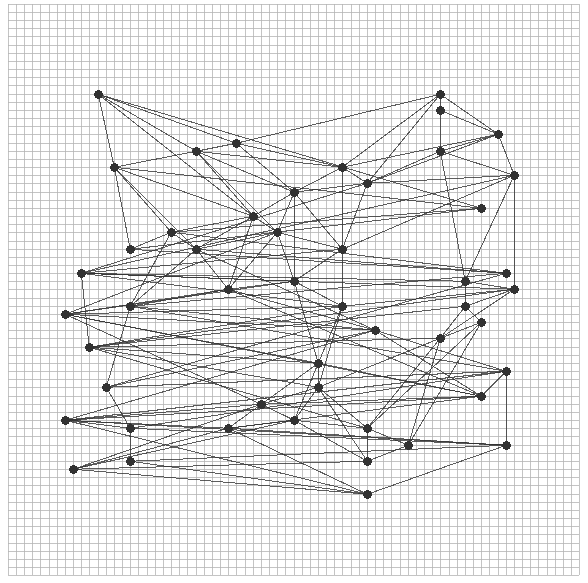
\includegraphics[width=6cm]{g5_initial.PNG}
\caption{Graph 5 initial output}
\end{minipage}
\begin{minipage}[t]{0.48\textwidth}
\centering
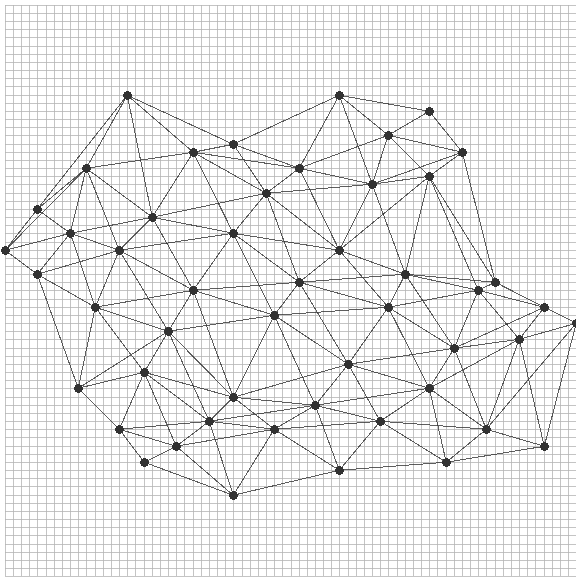
\includegraphics[width=6cm]{g5_FD.png}
\caption{Graph 5 after FD process}
\end{minipage}
\begin{minipage}[t]{0.48\textwidth}
\centering
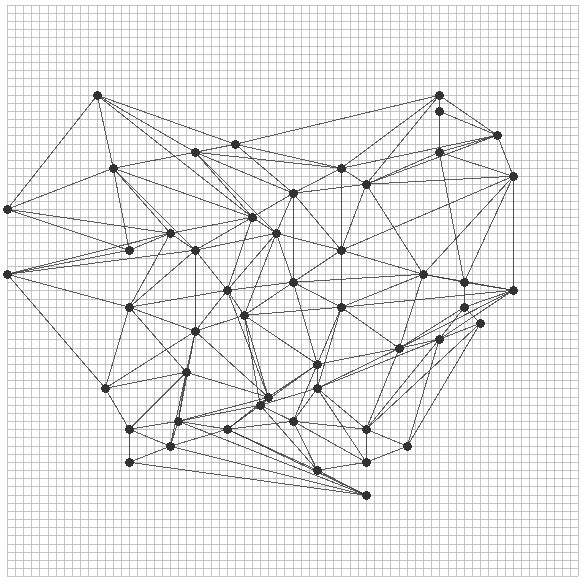
\includegraphics[width=6cm]{g5_LSNode.PNG}
\caption{Graph 5 after LS by nodes process}
\end{minipage}
\begin{minipage}[t]{0.48\textwidth}
\centering
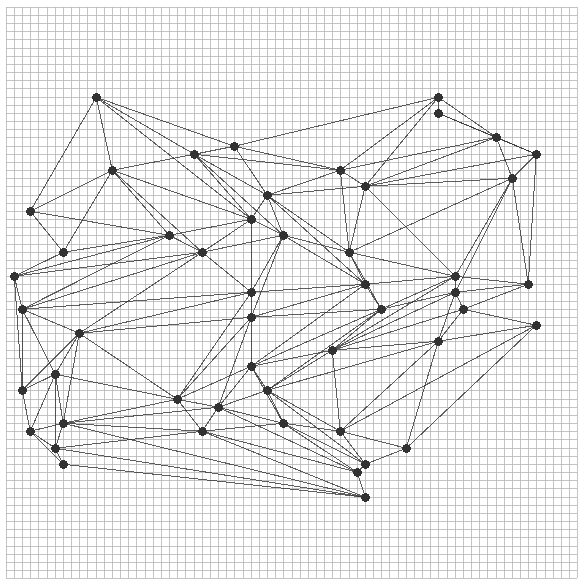
\includegraphics[width=6cm]{g5_LS.PNG}
\caption{Graph 5 after LS by edges process}
\end{minipage}
\end{figure}


\subsection{Time Complexity}

We use a similar table to show the time complexity of these three algorithms in different graph. As our algorithms does not do operations in $y$ axe so we will only look at the graph width. We will also only choose 5 examples with very different dimensions.

\begin{table}[h]
\centering
\begin{tabular}{ p{0.1\textwidth} | p{0.1\textwidth} | p{0.1\textwidth}| p{0.1\textwidth}| p{0.12\textwidth}| p{0.12\textwidth} | p{0.12\textwidth}}
     \hline
     Graph number & Width & Number of nodes & Number of edges & FD result (ms) & LS by nodes result (ms) & LS by edges result (ms)\\
     \hline
     \codeword{2} & 20 & 16 & 42 & 8 & 5 & 366 \\
     \hline
     \codeword{7} & 100000 & 100 & 150 & 120 & 16386 & 7941\\
     \hline
     \codeword{10} & 1000000 & 500 & 684 & 1197  & 190553 & 245671\\
     \hline
     \codeword{11} & 1000000 & 1800 & 6961 & 10724 & 4232 & 2533482\\
     \hline
\end{tabular}
\end{table}

The table tell us:
\begin{enumerate}
    \item The time complexity increase of the FD algorithm is the most stable. Even for large graphs, it can be solved in a reasonable time, but its results may not be very good.
    \item However, the LS by nodes algorithm increase quickly. But if, after a local optimization, the method detects that the results do not improve significantly, the program will end automatically like in Graph 11. It should be noted that although we also set the value of \lstinline{tol} for LS by edge algorithm, but here the \lstinline{tol} is used for step length which will by reduced if the number of intersections augment. Due to the randomness of this algorithm, the chance of not having improvement continuously in several local optimization is very low, so Graph 11 will converge quickly only for LS by nodes algorithm.
    \item The LS by edges algorithm always has a very high time complexity, and this complexity also gives it more outstanding performance.
\end{enumerate}


%bibliography
\newpage
\bibliography{ref.bib}
\bibliographystyle{apacite}

\end{document}


